\documentclass[11pt,wide]{mwart}

\usepackage{graphicx}

\usepackage{subcaption}
\usepackage{float}


\usepackage{amsmath,amssymb,amsfonts,amsthm,mathtools}

\usepackage{bbm}
\usepackage{hyperref}
\usepackage{url}
\usepackage[T1]{fontenc}
\usepackage[polish]{babel}
%\usepackage{comment}      

%\usepackage{csvsimple}
%\usepackage[section]{placeins}
\usepackage{tikz}
\usepackage{graphicx}

\graphicspath{ {./wykresy} }

\newtheorem{definition}{Definicja}[section]
\raggedbottom
\newcommand{\norm}[1]{\left\lVert#1\right\rVert}

\title{\LARGE\textbf{Pracownia 2 z analizy numerycznej}\\Zadanie 12}
\author{Wojciech Pokój 324526, Krzysztof Wasielewski 322091}
\date{Grudzień 2021}

\begin{document}

\maketitle

\section{Wstęp}
Rozkład macierzy jest narzędziem umożliwiającym przekształcenie macierzy do postaci iloczynu kilku macierzy o nowych właściwościach. Zagadnienie to ma zastosowanie w numerycznym rozwiązywaniu układów liniowych. Jednym z rozważanych rozkładów jest rozkład QR. Polega on na przedstawieniu macierzy wejściowej w postaci iloczynu macierzy ortonormalnej Q oraz macierzy górnotrójkątnej R. Stosowalność rozkładu QR w rozwiązywaniu układów równań liniowych wynika bezpośrednio z własności Q oraz R. Rozważmy układ
$$M\vec{x} = \vec{y}$$
Stosując rozkład QR
$$QR\vec{x} = \vec{y}$$
$$Q^{-1}QR\vec{x}=Q^{-1}\vec{y} $$
$$R\vec{x}=Q^{-1}\vec{y} $$
Ortonormalność Q oznacza, że zachodzi $Q^TQ=QQ^T=Id$, czyli $Q^{-1}=Q^T$. 
$$R\vec{x}=Q^T\vec{y}$$
Rozwiązanie takiego układu jest już proste, ponieważ po prawej stronie jest wektor wartości, a po lewej macierz górnotrójkątna przemnożona przez wektor niewiadomych. Można to zrobić metodą \textit{podstawiania wstecz}. 
W dalszej części przedstawimy metody otrzymywania takiego rozkładu.

\section{Algorytmy rozkładu QR}

Na początku dokładnie zdefiniujmy 3 algorytmy rozkładu QR które będziemy porównywać w dalszej części pracy.

\subsection{Metoda Grama - Schmidta}

Do znajdowania rozkładu $QR$ macierzy można się posłużyć faktem że macierz $Q$ jest macierzą ortonormalną (tj. $Q^TQ = Id$). Oznacza to że w tym celu można wykorzystać algorytm Grama - Schmidta do znajdowania ortogonalnej bazy dla macierzy $Q$.

Zastosujmy algorytm Grama - Schmidta dla macierzy $A = [ a_1 | a_2 | \dots | a_n]$.
Rzut prostopadły wektora $a$ na wektor $u$ definiujemy jako:
\begin{equation}
    proj_ua = \frac{\langle u ; a \rangle}{\langle u ; u \rangle} u
\end{equation}

Wtedy:
\begin{equation*}
\begin{aligned}[t]
& u_1 = a_1                                     & e_1 = \frac{u_1}{\norm{u_1}} \\
& u_2 = a_2 - proj_{u_1} a_2                    & e_2 = \frac{u_2}{\norm{u_2}} \\
& u_3 = a_3 - proj_{u_2} a_3 - proj_{u_1} a_3   & e_3 = \frac{u_3}{\norm{u_3}} \\
& \vdots                                        & \vdots \\
& u_n = a_n - \sum_{k = 0}^{n-1} proj_{u_k}a_n  & e_n = \frac{u_n}{\norm{u_n}}
\end{aligned}
\end{equation*}

Otrzymujemy w ten sposób ortogonalną bazę $U = \{u_1, u_2, \dots u_n\}$ oraz ortonormalną bazę  $E = \{e_1, e_2, \dots e_n\}$. Zauważmy, że wektory macierzy $A$ wyrażają się jako:

\begin{equation*}
\begin{aligned}
& a_1 = \langle e_1; a_1 \rangle e_1 \\
& a_2 = \langle e_1; a_2 \rangle e_1 + \langle e_2; a_2 \rangle e_2 \\
& a_3 = \langle e_1; a_3 \rangle e_1 + \langle e_2; a_3 \rangle e_2 + \langle e_3; a_3 \rangle e_3 \\
& \vdots \\
& a_n = \sum_{k = 0}^n \langle e_k; a_n \rangle e_k
\end{aligned}
\end{equation*}

Przy czym $ \langle e_i; a_i \rangle = \norm{u_i}$.

Stąd rozkład $QR$ macierzy $A$ wyraża się jako:

\begin{equation}
\begin{aligned}
Q = \begin{bmatrix} e_1 & e_2 & e_3 & \dots & e_n \end{bmatrix};
& R = \begin{bmatrix} 
\langle e_1; a_1 \rangle & \langle e_1; a_2 \rangle & \langle e_1; a_3 \rangle & \dots \\
                         & \langle e_2; a_2 \rangle & \langle e_2; a_3 \rangle & \dots \\
                         &                          & \langle e_3; a_3 \rangle & \dots \\
\vdots & \vdots & \vdots & \ddots
\end{bmatrix}
\end{aligned}
\end{equation}
Gdzie macierz $Q$ jest macierzą ortogonalną, a $R$ macierzą górnotrójkątną.

\subsection{Zmodyfikowany algorytm Grama - Schmidta}

Algorytm Grama - Schmidta jest bardzo prosty ale też jest niestabilny numerycznie. Błąd w wyliczaniu $k$-tego wektora bazy ortogonalnej będzie się przenosić na wszystkie kolejne wektory, stąd ostatni wektor jest najbardziej zaburzony i nieprecyzyjny. 
Na bazie oryginalnego algorytmu opracowano równoważny mu algorytm, ale bardziej stabilny.
Zamiast obliczać $k$-ty wektor jako różnicę wektora i jego rzutów na dotychczas policzonej bazie, stosuje się wzór rekurencyjny:

\begin{equation*}
\begin{aligned}[t]
& u_k^{(1)} = a_k - proj_{u_1} a_k \\
& u_k^{(2)} = u_k^{(1)} - proj_{u_2} u_k^{(1)} \\
& \vdots \\
& u_k^{(k-2)} = u_k^{(k-3)} - proj_{u_{k-2}} u_k^{(k-3)} \\
& u_k^{(k-1)} = u_k^{(k-2)} - proj_{u_{k-1}} u_k^{(k-2)} \\
& e_k = \frac{u_k^{(k-1)}}{\norm{u_k^{(k-1)}}}
\end{aligned}
\end{equation*}

Gdzie $U = \{u_1, u_2^{(1)}, \dots u_n^{(n-1)}\}$ jest bazą ortogonalną, a $E = \{e_1, e_2, \dots e_n\}$ odpowiadającą bazą ortonormalną.

Różnica polega na tym, że zamiast w jednej iteracji wyliczyć nowy wektor, stopniowo ortogonalizuje się resztę bazy. W arytmetyce o skończonej precyzji błędy kumulując się dużo wolniej i w mniejszym stopniu zaburzają wynik dokładny. Niestety algorytm w całości nie emliminuje niekorzystnego zjawiska kumulacji błędu, ale na pewno pomaga go ograniczyć.

\subsection{Metoda Householdera}

Do rozłożenia macierzy $M$ do postaci $QR$ rozważmy następujący ciąg transformacji:
 $$H_n \dots H_1 M = R$$
Macierze $H_i$ mają za zadanie sprowadzić macierz $M$ do postaci górnotrójkątnej przez zerowanie współczynników M, które znajdują się pod przekątną. Oznacza to, że po kolejnych mnożeniach zachodzi
$$M= \begin{bmatrix} 
 m & m & \dots&m\\
 \vdots&& &\\
 m & m & &m\\
\end{bmatrix}$$
$$H_1 M= \begin{bmatrix} 
 m & m & \dots&m\\
 0 & \bar{m} & &\bar{m}\\
 \vdots&& &\\
 0 & \bar{m}& &\bar{m}\\
\end{bmatrix}$$
$$H_2H_1 M= \begin{bmatrix} 
 m & m & \dots&m\\
 0 & \bar{m} & &\bar{m}\\
  0 & 0 & &\tilde{m}\\
 \vdots&& &\\
 0 & 0& &\tilde{m}\\
\end{bmatrix}$$
Poszukiwane macierze $H_i$ muszą być ortonormalne, tak by ich iloczyn również posiadał tę właściwość. Macierze te mają zachowywać już przetworzone wiersze, dlatego będą miały strukturę
$$H_i= \begin{bmatrix} 
Id_{i-1}& 0\\
0& F_i\\
\end{bmatrix}$$
gdzie $F_i$ jest macierzą odpowiedzialną za wspomniane już zerowanie współczynników. Na rysunku poniżej przedstawiony jest przypadek dwuwymiarowy, w którym wektor $u$ jest transformowany na kierunek wektora bazowego $e_1$.  Wektor $v$ jest dobrany w ten sposób, że $v  = \norm{u}e_1-u$. Szukamy $F_i$ spełniającego $F_iu = \norm{u}e_i$. Zauważyć można, że $F_i$ będzie bardzo podobne do rzutu prostopadłego na płaszczyznę $H$ wyrażonego przez $P=Id-\frac{1}{v^Tv}vv^t$. Jedyną różnicą jest podwojenie odejmnika, stąd $F_i =\frac{2}{v^Tv}vv^t $
\begin{figure}[H]
\centering
\begin{tikzpicture}
  \draw[thin,gray!40] (0,0) grid (6,5);
  \draw[<->] (0,0)--(0,5) node[right]{$e_2$};
  \draw[<->] (0,0)--(6,0) node[above]{$e_1$};
  \draw[line width=2pt,blue,-stealth](0,0)--(2,4) node[anchor=south west]{$\boldsymbol{u}$};
  \draw[line width=2pt,blue,-stealth](0,0)--(4.5,0) node[anchor=north west]{$\boldsymbol{u'}$};
  
   
    \draw[line width=1pt,green,-stealth](0,0)--(6,3.69) node[anchor=north west]{$\boldsymbol{H}$};
    \draw[line width=2pt,red,-stealth](2,4)--(4.5,0) node[anchor=south west]{$\boldsymbol{v}$};
  
\end{tikzpicture}
\caption{Transformacja wektora $u$ na kierunek wektora bazowego $e_1$} \label{C1}
\end{figure}
$F_i$ rzeczywiście jest macierzą ortonormalną, bo $F_i^TF_i= Id - 4\frac{1}{v^Tv}vv^t+4\frac{1}{v^Tv}vv^t\frac{1}{v^Tv}vv^t=Id$
\\ Mając już ciąg macierzy $H_i$ można uzyskać $Q^T$ biorąc ich iloczyn. Macierz $R$ powstaje przez zaaplikowanie $Q^T$ do wejściowej macierzy $M$.
%Macierz transformacji Housenholdera $H=Id-\frac{2}{v^Tv}vv^t$ odpowiada operacji odbijania wektora względem płaszczyzny prostopadłej do $v$. Posłużymy się tą własnością do znalezienia rozkładu QR\\
%Metoda ta konstuuje ciąg macierzy $H_i$ taki, że $$H_n \dots H_1 M = R$$ gdzie $M$ jest macierzą początkową, a $R$ górnotrójkątną. Każda z macierzy $H_i$ dobrana jest tak, żeby zerowała współczynniki w kolejnych kolumnach $M$, które znajdują się pod przekątną. Takie macierze można zapisać w postaci $$H_i= \begin{bmatrix} 
% Id_{i-1}& 0\\
% 0& H_i'\\
%\end{bmatrix}$$ gdzie $H_i'$ spełnia $H_i' a_i = |a_i|e_i$. $H_i'$ jest po prostu macierzą Housenholdera dla $v = a_i-|a_i|e_i$. Macierz $Q$ jest wówczas iloczynem macierzy $H_i$.

\section{Testowanie metod}
\subsection{Stabilność numeryczna}

Jednym z najważniejszych zagadnienień do rozpatrzenia to stabilność numeryczna podanych algorytmów, czyli jak niewielkie zmiany będą wpływać na wynik dokładny. W arytmetyce o nieskończonej precyzji zachodzi że dla dwóch różnych macierzy i dowolnego algorytmu rozkładu QR: 
\begin{equation}
M - Q_MR_M = M' - Q_{M'}R_{M'} = 0
\end{equation}

Jeżeli maciecz $M$ zaburzymy o $\Delta M$, gdzie wartości nie przekraczają w module pewnego ustalonego dowolnie małego $\epsilon$ to algorytm powinien dla $M' = M + \Delta M$ zwracać nieznacznie zaburzony wynik względem macierzy $M$. Algorytmy stabilniejsze numerycznie powinny lepiej sobie radzić z zaburzeniami danych niż te niestabilne numerycznie. Porównanie dwóch algorytmów $A_1$ i $A_2$ będziemy wykonywać przez ustalenie pewnej macierzy $M$, jej zaburzenia $\Delta M$ i sprawdzenia która z metod da mniejszy błąd E:

\begin{equation}
\begin{aligned}
    & E(A_n, M, M') := M - A_n(M) - (M' - A_n(M')) \\
    & A_n(M) := Q_M^{(A_n)}R_M^{(A_n)}
\end{aligned}
\end{equation}

Żeby porównać 2 macierze potrzeba jest do zdefiniowana norma która pozwoli ocenić która z macierzy jest mniejsza. W naszym przypadku za normę posłuży średnia arytmetyczna wszystkich współczynników macierzy w module:

\begin{equation}
\norm{E} = \frac{1}{nm}\sum_{i=0}^n\sum_{j=0}^m |e_{ij}|
\end{equation}

Testy stabilności numerycznej wykonano przez wylosowanie macierzy 10x10 o promieniu losowości współczynników nie przekraczającym 100, a następnie stopniowym dodawanie zaburzeń i porównywaniu błędów kolejnych zaburzonych macierzy. Testy powtarzano kilkukrotnie i łatwo można było zauważyć że wykresy rzędów błędów w kolejnych iteracjach wpadają w 2 główne schematy:

\begin{enumerate}
    \item Metoda Householdera zaznaczona na zielono jest lepsza, niż reszta metod i kolejne błędy formują stabilną krzywą oscylującą wokół $y = -14$. Z kolei Podstawowa metoda Grama-Schmidta okazauje się lepsza niż zmodyfikowana wersja czasem nawet o cały rząd wielkości. Warto zauważyć że wykresy dla obu wersji ma mniej więcej ten sam kształt, przynajmniej charakterystyczne nagłe wzrosty i spadki jakości obliczeń są zauważalne się w obu wykresach w tych samych miejscach.
    
    \vspace{1cm}
    \centerline{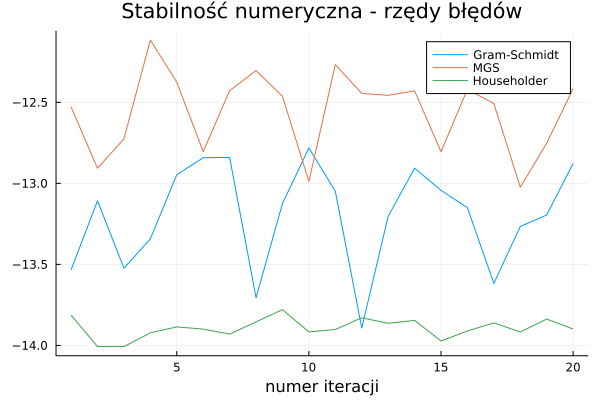
\includegraphics[scale=0.6]{stability2}}
    
    \item Wykresy są chaotyczne, metoda Householdera i algorytm Grama-Schmidta wzajemnie się przeplatają lub wręcz Gram-Schmidt genruje mniejsze błędy. Metoda Householdera za każdym razem formuje krzywą wokół prostej $y = -13.9$. Pomimo tego że Gram-Schmidt jakością dorównuje lub przewyższa metodę Householdera, zmodyfikowany algorytm Grama-Schmidta ciągle jest wyraźnie gorszy niż wersja podstawowa.
    
    \vspace{1cm}
    \centerline{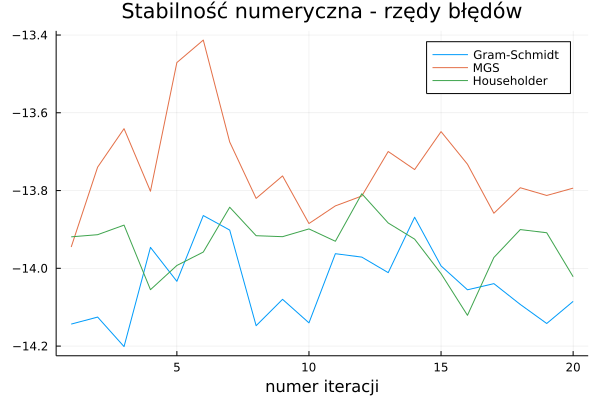
\includegraphics[scale=0.6]{stability1}}
    
\end{enumerate}

Takie wyniki dobrze wskazują na kilka cech rozważanych algorytmów:
\newline
\begin{itemize}
    \item Metoda Householdera jest najstabilniejsza ze wszystkich metod, praktycznie zawsze rząd błędu jest niegorszy niż $-14$. W wykresie nie występują drastyczne zmiany tego błędu.
    \newline
    \item Metoda Grama-Schmidta jest ogólnie gorsza niż metoda Householdera, okazjonalnie potrafi uzyskać lepszą dokładność, ale jest to okupione niestabilnym wykresem. Czasem drobne perturbacje danych zmieniają dyrastycznie uzyskiwane wyniki.
    \newline
    \item Zmodyfikowany algorytm Grama-Schmidta uzysuje praktycznie zawsze gorszą dokładność niż podstawowa wersja. Wykres z reguły jest bardzo podobny dla podstawowej metody, co jest spodziewanym wynikiem, ponieważ obie metody są sobie algorytmicznie równoważne. Na uwagę zasługuje fakt że pomimo gorszych wyników wykresy mają mniejszą amplitudę niż wersja podstawowa. Oznacza to że rzeczywiście zmodyfikowany algorytm jest stabilniejszy numerycznie.
    \newline
\end{itemize}



\subsection{Dokładność a rozmiar macierzy}

Innym zagadnieniem jest sprawdzenie jak dobrze algorytmy radzą sobie z rozkładem QR gdy rośnie rozmiar macierzy. Tutaj znowu przewagę będą mieć algorytmy stabilniejsze numerycznie, ponieważ z założenia będą kumulować błędy wolniej i w mniejszym stopniu, dzięki czemu wyniki dla końcowych iteracji będą na ogół dokładniejsze. Tutaj metodą testowania będzie porównanie średniego błędu dla zbioru losowych macierzy wraz ze zwiększaniem rozmiaru macierzy.

W tym teście rozpatrywana będzie średnia dokładność dla 20 losowych macierzy o promieniu losowości równym $5$ dla każdego algorytmu i stopniowe zwiększanie rozmiaru losowanych macierzy z 3x3 na 30x30. 

W przeciwieństwie do poprzedniego podpunktu, tutaj wykresy wpadają w tylko jeden scenariusz.

\vspace{1cm}
\centerline{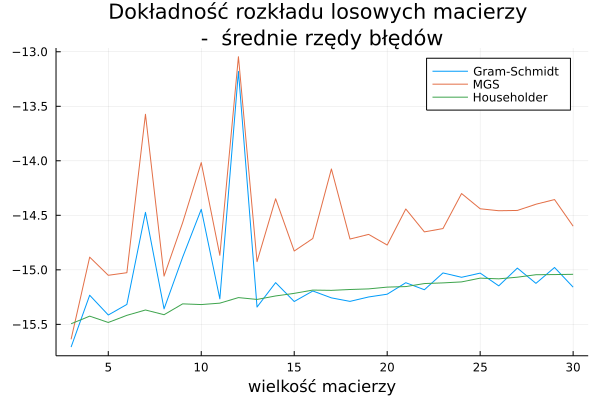
\includegraphics[scale=0.6]{random6}}
\vspace{1cm}
\centerline{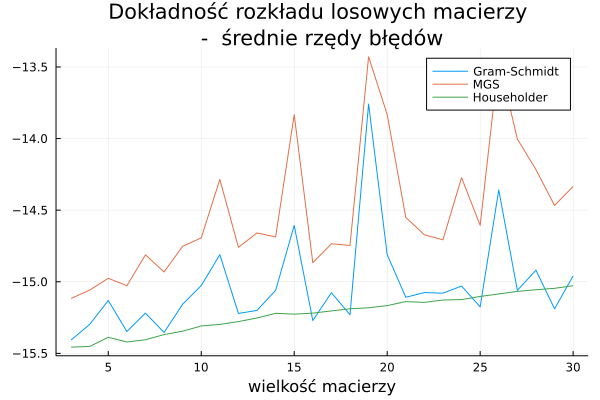
\includegraphics[scale=0.6]{random3}}

\begin{itemize}
    \item Błędy dla metoda Householdera powoli i stabilnie rosną między od $-15.5$ do $-15$.
    \newline
    
    \item Metoda Grama-Schmidta wydaje się podążać tym samym trendem co metoda Houseoldera, ale dużo mniej stablinie. Okazjonalnie pojawiają się nagłe pogorszenia jakości, co może oznaczać że w próbie badawczej znalazło się kilka macierzy dla których ortogonalizacja była źle uwarunkowana.
    \newline
    
    \item Zmodyfikowany algorytm Grama-Schmidta odzwierciedła dokładnie zachowanie zwykłego algorytmu, ale z gorszym błędem o około cały rząd wielkości. W niewielkim tylko stopniu algorytm ma gładszy wykres niż podstawowa wersja, co oznacza że nie ma zbyt wielkiego zysku z tego algorytmu w sytuacji o jednej próbie badawczej, gdzie stabilność nie ma takiego znaczenia.
    \newline
    
\end{itemize}

\subsection{Zakres współczynników macierzy a poprawność rozwiązania}
Ponieważ rozkład QR jest istotny dla problemu rozwiązywania układów liniowych. Dlatego dla wygenerowanych losowo układów liniowych ze współczynnikami z coraz większego zakresu wykonano porównanie metod. Dla każdej metody rozkładu QR wyliczono średnią różnicę między rozwiązaniami uzyskanymi z metody podstawiania wstecz, a wartościami wykorzystanymi do wygenerowania układu.

\vspace{1cm}
\centerline{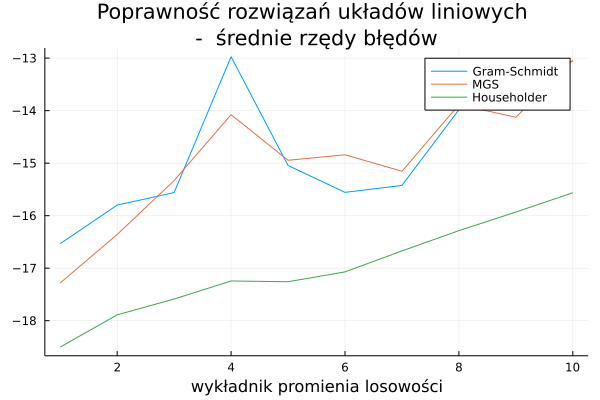
\includegraphics[scale=0.6]{linear6}}

Ponownie metoda Householdera okazała się najbardziej stabilna. Metoda Grama-Schmidta w standardowej wersji sprawowała się bardzo podobnie do jej zmodyfikowanego wariantu. Zyski ze zmodyfikowanego algorytmu Grama-Schmidta praktycznie nie są odczuwalne.


\section{Wnioski}

Szereg testów wykonanych na podanych metodach jednoznacznie wskazują, że metoda Householdera jest najlepsza pod każdym względem ze wszystkich. Cechuje ją najlepsza stabilność numeryczna i duża dokładność uzyskiwanych wyników. Największy problem tego algorytmu to duża złożoność obliczeniowa i brak możliwości pararelizowania obliczeń. Każda iteracja zmienia wszystkie współczynniki potrzebne w następnych iteracjach obliczeń. Do tego wymagane jest wymnażanie macierzy $O(n)$ razy co może być odczuwalne w przypadku większych macierzy.

Metoda Grama-Schmidta jest gorsza od metody Householdera, tylko w nielicznych przypadkach potrafi osiągnąć lepszą dokładność niż metoda Householdera, ale różnice nie przekraczają nawet połowy rzędu wielkości. Niestety w większości sytuacji metoda zachowuje się bardzo nieprzewidywalnie. Testy pokazują że metoda potrafi zachowywać się dość chaotycznie i nagle może nastąpić utrata cyfr znaczących. Do zalet tej metody należy fakt że jest oparta na bardzo łatwym iteracyjnym algorytmie ortogonalizacji, który w przeciwieństwie do metody Householdera, można zrównoleglić.

Zmodyfikowany algorytm Grama-Schmidta okazał się najmniej dokładny ze wszystkich przedstawianych metod. Zwykła metoda często okazuje się być dokładniejsza o cały rząd wielkości. Przeprowadzone testy pokazują że wersja zmodyfikowana i podstawowa są sobie bardzo zbliżone. Wykresy obu metod zachowują ten sam kształt, z tym że zmodyfikowany algorytm nieznacznie te wykresy wygładza co świadczy o lepszej stabilności numerycznej tego rozwiązania.

\section{Literatura}

\begin{enumerate}
	\item D. Kincaid, W. Cheney, \textit{Analiza numeryczna}, WNT, 2005.
	\item Wikipedia, \textit{\href{https://en.wikipedia.org/wiki/QR_decomposition}{QR Decomposition}}
	\item Wikipedia, \textit{\href{https://en.wikipedia.org/wiki/Gram\%E2\%80\%93Schmidt_process}{Gram-Schmidt process}} 
\end{enumerate}

\end{document}
